% robust-ms-gate.tex — REVTeX 4.2 port of docs/robust-ms-gate-manuscript.md
% Compile: pdflatex; bibtex; pdflatex; pdflatex   (needs references.bib, figures/)
% DRAFT v0.1 — quantitative results marked as measured; author block is a placeholder.
\documentclass[aps,prapplied,twocolumn,superscriptaddress,floatfix,nofootinbib]{revtex4-2}
\usepackage{amsmath,amssymb}
\usepackage{graphicx}
\usepackage{bm}
\graphicspath{{figures/}}

\begin{document}

\title{Analytic design and open-system verification of robust M\o lmer--S\o rensen
gates: quantifying the coherent--incoherent trade-off}

\author{Siridech B.}
\email{siridech.bo@kmitl.ac.th}
\affiliation{King Mongkut's Institute of Technology Ladkrabang (KMITL), Bangkok, Thailand}
% Placeholder author block — finalize before submission.

\begin{abstract}
Robust M\o lmer--S\o rensen (MS) gates are designed almost exclusively against
\emph{coherent} error, while the \emph{incoherent} environment (motional heating,
dephasing, spontaneous emission during the gate) is treated separately. Because the
leading robust-control techniques necessarily extend the gate time, coherent-error
suppression is bought at the price of increased incoherent accumulation. We present a
cross-validated toolchain that couples a fast \emph{analytic} MS designer/verifier
(second-order Magnus in the commuting $\sigma_x$ basis, $O(M)$ per gate for $M$ modes)
to a \emph{full open-system} Lindblad integrator carrying the same parameters. We
(i)~confirm the two engines agree to $\sim\!3\times10^{-9}$ in Bell-state infidelity in
the closed-system limit; (ii)~reproduce the coherent robustness of the symmetric-robust
($2.5\times10^{3}\times$ suppression of the symmetric-drift residual) and generator-based
compensation (GBC, $\varepsilon^2\!\to\!\varepsilon^4$) schemes; and (iii)~map the
coherent--incoherent trade-off: GBC's $\varepsilon^4$ advantage costs a $\approx\!4\times$
gate time (hence $\approx\!4\times$ incoherent error), so a crossover asymmetric detuning
$\Delta\omega^\times$ separates a regime where the single robust gate wins from one where
GBC wins. $\Delta\omega^\times$ grows monotonically with the incoherent floor as
$\Delta\omega^\times\!\propto\!\sqrt{I_{\rm incoh}}$, giving a direct rule for when
pulse-shaping complexity pays off under real trap noise. The trade-off is
species-independent (identical for ${}^{40}$Ca$^+$ and ${}^{171}$Yb$^+$ in dimensionless
units), a consequence of fixed $\eta\Omega$ at loop closure.
\end{abstract}

\maketitle

\section{Introduction}
Trapped ions are among the leading platforms for quantum computation, with two-qubit MS
fidelities above $99.9\%$~\cite{Ballance16,Gaebler16,Clark21}. Coherent control error
splits, following the red/blue-tone geometry of the bichromatic drive, into a
\emph{symmetric} error (both sidebands shift together, a motional-detuning drift, an
unclosed phase-space trajectory) and an \emph{asymmetric} error (the tones shift
oppositely, a drift of the qubit center line, a $\sigma_z$ rotation on both qubits). The
former is suppressed by robust waveforms~\cite{Leung18,Milne20,Roos08,Zhu06}; the latter
does not commute with the entangler $G=\sigma_x^{j_1}\sigma_x^{j_2}$ and was recently
addressed by generator-based compensation (GBC)~\cite{Zhang25}, which cancels the residual
$\sigma_z$ to first order at the cost of a doubled-gate-time segment. For ${}^{40}$Ca$^+$,
asymmetric error is the second-largest error source~\cite{Pogorelov21,Postler22}.

All of this is validated in the closed-system limit, yet every robustness technique
\emph{lengthens the gate}, and longer gates accumulate more incoherent error. We ask:
\emph{how much of the coherent robustness survives realistic dissipation, and where is
the net-fidelity optimum?} Answering it requires one framework that both designs the
robust coherent pulse and verifies it under the full master equation. The analytic core
we use is established~\cite{Sorensen00,Leung18,Zhang25} and we claim no novelty for it;
our contributions are (N1)~a unified design$\to$open-system-verify pipeline,
(N2)~the quantitative coherent--incoherent trade-off map, and (N3)~its extension toward
$N\!\le\!4$-ion chains.

\section{Theoretical framework}
\subsection{Ideal multi-mode MS Hamiltonian}
In the Lamb--Dicke and rotating-wave approximations,
\begin{equation}
\hat H_{\rm int}(t)=\tfrac12\Omega(t)\sum_{j,m}\eta_m b^m_j\,\sigma_x^j
\big(a_m^\dagger e^{i\delta_m t}+a_m e^{-i\delta_m t}\big).
\end{equation}
The coupling operators all commute, so the second-order Magnus expansion terminates:
\begin{equation}
\hat U(\tau)=\exp\!\Big[i\Theta\,\sigma_x^{j_1}\sigma_x^{j_2}
-\tfrac{i}{2}\!\sum_{j,m}(\alpha_m a_m^\dagger+\alpha_m^* a_m)\eta_m b^m_j\sigma_x^j\Big],
\end{equation}
\begin{equation}
\alpha_m(\tau)=\!\int_0^\tau\!\Omega\,e^{i\delta_m t}dt,\quad
\Theta=\tfrac12\!\sum_m\eta_m^2 b^m_{j_1}b^m_{j_2}\!\!\iint\!\Omega\Omega\sin[\delta_m(t_1{-}t_2)].
\end{equation}
The gate is clean when $\alpha_m(\tau)=0$ and $\Theta=\pi/4$.

\subsection{Coherent errors and robust waveform}
A common-mode asymmetric error adds $\tfrac{\Delta\omega}{2}\sum_j\sigma_z^j$. Imposing a
symmetric pulse $\Omega(t)=\Omega(\tau-t)$ and $\int_0^\tau\alpha_m\,dt=0$ gives closure,
first-order insensitivity $\partial_{\delta_m}\alpha_m=0$, and $\beta_m(\tau)=0$, collapsing
the operator to the motion-free form
\begin{equation}
\hat U(\tau)=\exp\!\Big[i\Theta\,\sigma_x^{j_1}\sigma_x^{j_2}-\tfrac{i}{2}\Delta\omega\tau\!\sum_j\sigma_z^j\Big].
\label{eq:star}
\end{equation}
The piecewise-constant robust waveform solves $A\mathbf{x}=\mathbf 0$ (closure),
$\mathbf{x}^{\mathsf T}M\mathbf{x}=\Xi$ (angle), with the minimum-intensity, sign-correct
solution $\mathbf{x}=\sqrt{\Xi/\lambda}\,\ker(A)\mathbf v_\lambda$~\cite{Zhang25,Leung18}.

\subsection{Generator-based compensation}
The residual $\varepsilon\equiv\Delta\omega\tau$ term in Eq.~\eqref{eq:star} does not
commute with $G$. GBC realizes the first-order-exact three-gate sequence
$\hat U^{\rm gbc}_\varepsilon=\hat U_\varepsilon\hat U^\dagger_{2\varepsilon}\hat U_\varepsilon
=\hat U_{\rm ideal}+o(\varepsilon^2)$, with $\hat U^\dagger_{2\varepsilon}=\hat\Pi\,\hat
U_{2\varepsilon}(-\Theta)\,\hat\Pi$ and $\hat\Pi=\sigma_x\!\otimes\!\sigma_x$; because
Eq.~\eqref{eq:star} is motion-free, this lives in the two-qubit ($4\times4$) space. The
residual infidelity is $O(\varepsilon^4)$ (GBC) vs $O(\varepsilon^2)$ (uncompensated).

\subsection{Open-system model (this work)}
We evolve the full $\rho$ on $\mathbb C^{2^N}\!\otimes\!\prod_m\mathcal F_m$ under
$\dot\rho=-i[\hat H(t),\rho]+\sum_c(L_c\rho L_c^\dagger-\tfrac12\{L_c^\dagger L_c,\rho\})$
with heating $L^-=\sqrt{\kappa(\bar n{+}1)}a_m$, $L^+=\sqrt{\kappa\bar n}a_m^\dagger$,
dephasing $\sqrt{\gamma_\phi/2}\,\sigma_z^j$, and decay $\sqrt{\Gamma}\,\sigma_-^j$ --- the
layer the coherent robust-control literature omits.

\section{Toolchain}
\begin{figure}[t]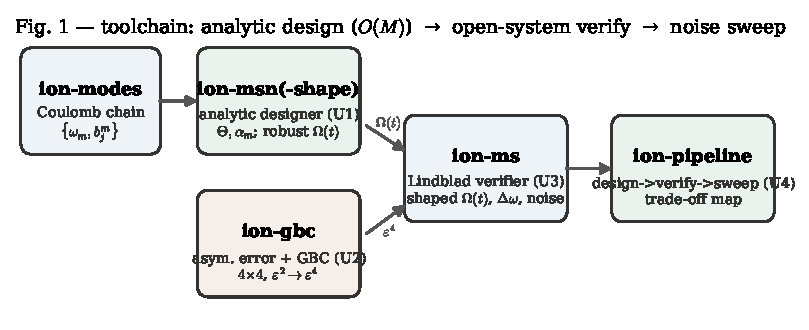
\includegraphics[width=\columnwidth]{Fig1_toolchain}
\caption{The design$\to$verify$\to$sweep toolchain (module names, upgrade tags U1--U4).}
\label{fig:toolchain}\end{figure}
The framework-free modules (Fig.~\ref{fig:toolchain}) are: \textsf{ion-msn(-shape)} ---
the $O(M)$ analytic designer ($\Theta$, $\alpha_m$, closure, robust $\Omega(t)$);
\textsf{ion-gbc} --- the $4\times4$ asymmetric-error/GBC gate; \textsf{ion-ms} --- the
full Lindblad integrator (piecewise $\Omega(t)$, $\Delta\omega$, noise); \textsf{ion-modes}
--- the Coulomb chain mode spectrum; \textsf{ion-pipeline} --- the sweep driver.

\section{Validation}
\begin{figure}[t]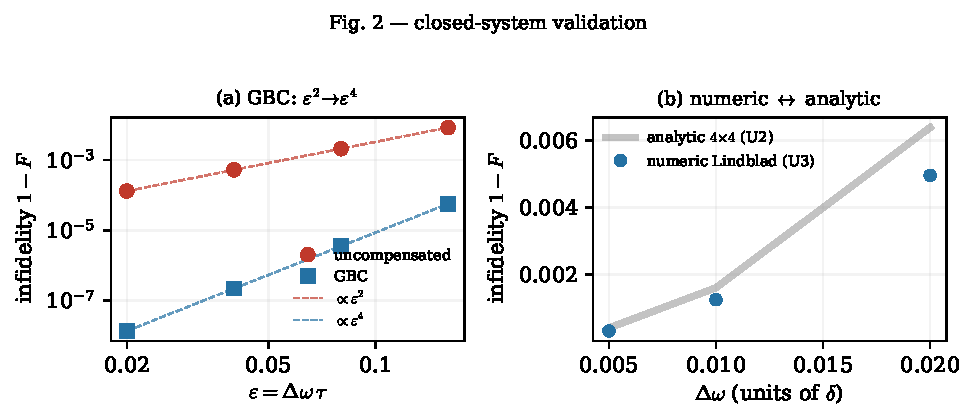
\includegraphics[width=\columnwidth]{Fig2_validation}
\caption{Closed-system validation: (a)~GBC turns the $\varepsilon^2$ asymmetric-error
infidelity into $\varepsilon^4$ (ratios $4.00$/$15.97$ per doubling); (b)~the numerical
Lindblad gate (U3) and the analytic $4\times4$ gate (U2) agree on the $\Delta\omega$-error
infidelity.}\label{fig:val}\end{figure}
In the closed-system limit the analytic and numerical Bell fidelities agree to
$|\Delta F|\approx3\times10^{-9}$. Fig.~\ref{fig:val} reproduces the $\varepsilon^2$ vs
$\varepsilon^4$ scaling~\cite{Zhang25} and the numeric$\leftrightarrow$analytic agreement.

\section{Numerical experiments}
Single-mode MS gate, $\eta=0.1$ (${}^{40}$Ca$^+$; $\nu_z=1$~MHz $\Rightarrow\eta\approx0.097$,
matching~\cite{Zhang25}), $\delta\equiv1$ (frequency unit), $K=1$, $N_{\rm Fock}=18$.

\textit{Method (validated-component decomposition).} GBC reaches $\varepsilon^4$ only when
$\beta_m=0$ (robust waveform); a constant single-mode drive has $\int\alpha\,dt\neq0$, so a
constant-leg GBC cancels only to $\varepsilon^2$. We therefore take GBC's coherent part from
the analytic gate ($\varepsilon^4$) and its incoherent part from the numerically integrated
$4\tau$ sequence at $\Delta\omega=0$, combined additively to leading order.

\paragraph{E1 --- incoherent baseline.} GBC's incoherent infidelity is $\approx4\times$ the
single gate across heating rates (Fig.~\ref{fig:e1}), its $4\tau$ vs $\tau$ cost.

\paragraph{E2 --- trade-off curve.} At fixed noise the single gate rises $\propto\Delta\omega^2$
while GBC sits at its incoherent floor; they cross at $\Delta\omega^\times$
(Fig.~\ref{fig:e2}).

\paragraph{E3 --- trade-off map.} $\Delta\omega^\times$ grows monotonically with the
incoherent floor (Table~\ref{tab:e3}, Fig.~\ref{fig:e3}), scaling as
$\sqrt{I_{\rm incoh}}$ since $\varepsilon^2(\Delta\omega^\times)\!\sim\!3I_{\rm incoh}$.
Repeating for ${}^{40}$Ca$^+$ ($\eta=0.10$) and ${}^{171}$Yb$^+$-Raman ($\eta=0.19$) gives
\emph{identical} crossovers; only the drive differs ($\Omega_{\rm closure}=5.0$ vs $2.6$,
$\propto1/\eta$), because $\eta\Omega=\delta/(2\sqrt K)$ is fixed at closure.

\begin{figure}[t]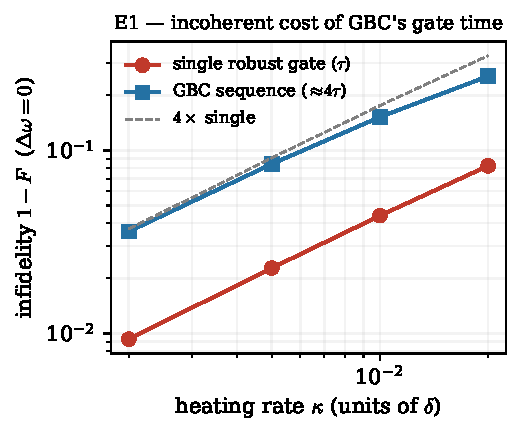
\includegraphics[width=0.86\columnwidth]{Fig3_E1_incoherent}
\caption{E1: GBC's $\approx4\tau$ incoherent cost vs heating $\kappa$.}\label{fig:e1}\end{figure}
\begin{figure}[t]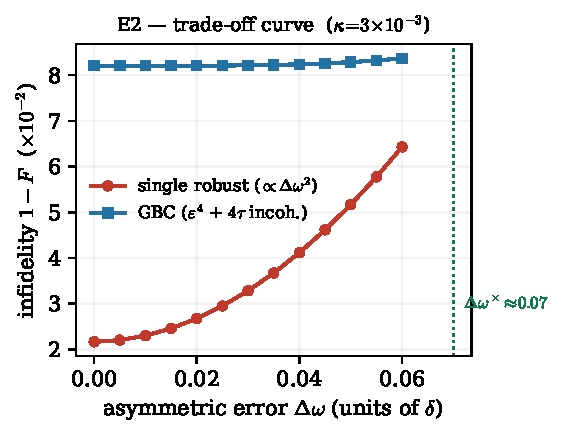
\includegraphics[width=0.86\columnwidth]{Fig4_E2_tradeoff}
\caption{E2: trade-off curve; crossover $\Delta\omega^\times\!\approx\!0.07$.}\label{fig:e2}\end{figure}
\begin{figure}[t]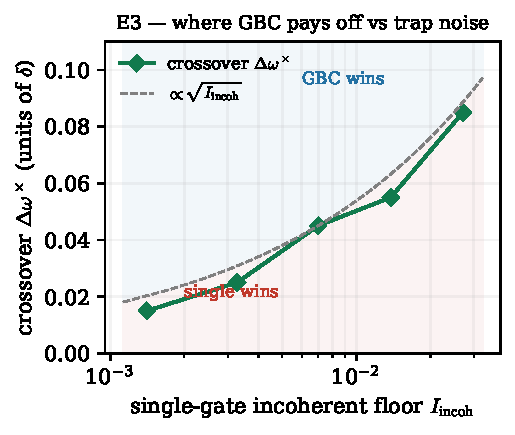
\includegraphics[width=0.86\columnwidth]{Fig5_E3_crossover}
\caption{E3: crossover $\Delta\omega^\times$ vs incoherent floor, $\propto\sqrt{I}$.}\label{fig:e3}\end{figure}

\begin{table}[t]\caption{E3 crossover vs heating $\kappa$ ($\bar n_{\rm th}=1$).}\label{tab:e3}
\begin{ruledtabular}\begin{tabular}{cccc}
$\kappa$ & single incoh. & GBC incoh. & $\Delta\omega^\times$ \\ \hline
$3\times10^{-4}$ & $1.4\times10^{-3}$ & $5.6\times10^{-3}$ & $0.015$ \\
$7\times10^{-4}$ & $3.3\times10^{-3}$ & $1.3\times10^{-2}$ & $0.025$ \\
$1.5\times10^{-3}$ & $7.0\times10^{-3}$ & $2.7\times10^{-2}$ & $0.045$ \\
$3\times10^{-3}$ & $1.4\times10^{-2}$ & $5.3\times10^{-2}$ & $0.055$ \\
$6\times10^{-3}$ & $2.7\times10^{-2}$ & $9.9\times10^{-2}$ & $0.085$ \\
\end{tabular}\end{ruledtabular}\end{table}

\section{Discussion}
The closed-system agreement between an $O(M)$ analytic engine and a full Lindblad
integrator makes design cheap and verification trustworthy. Robust waveforms and GBC
trade coherent suppression for gate time, so their benefit is conditional on the
incoherent budget: below $\Delta\omega^\times$ use the single robust gate; above it, GBC.
\emph{Limitations.} The analytic operator is second-order Magnus~\cite{Zhang25}; the
Lindblad study is single-mode ($N\!\le\!4$ multi-mode deferred); the beyond-RWA carrier is
a leading-order estimate; and a fully-coupled shaped-leg numerical GBC (needing
$N_{\rm Fock}\!\gtrsim\!30$ and sub-$\varepsilon^2$ leg calibration) remains open.

\section{Conclusion}
We provide a design$\to$open-system-verify toolchain for robust MS gates and quantify the
coherent--incoherent trade-off that governs whether robust-control gains survive
dissipation --- a direct rule ($\Delta\omega^\times\!\propto\!\sqrt{I_{\rm incoh}}$,
species-independent) for when pulse-shaping complexity pays off.

\begin{acknowledgments}
CiRA QuantumSim (KMITL). Software cross-validated against the analytic framework
of~\cite{Zhang25}.
\end{acknowledgments}

\bibliographystyle{apsrev4-2}
\bibliography{references}

\end{document}
